\newpage
\section{The Manaworld examples}
%\FloatBarrier
\begin{table}
  %~ \begin{center}
		\begin{tabular}{c c}
		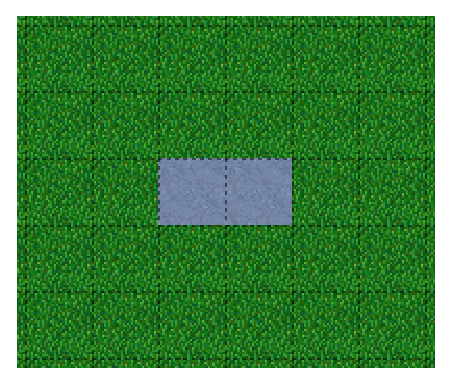
\includegraphics[scale=1]{Example/TheManaWorld/flow1.eps} &
	    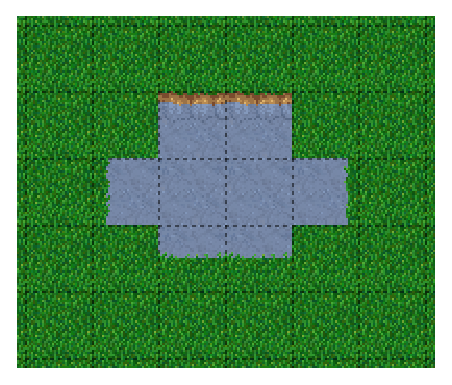
\includegraphics[scale=1]{Example/TheManaWorld/flow2.eps} \\
	    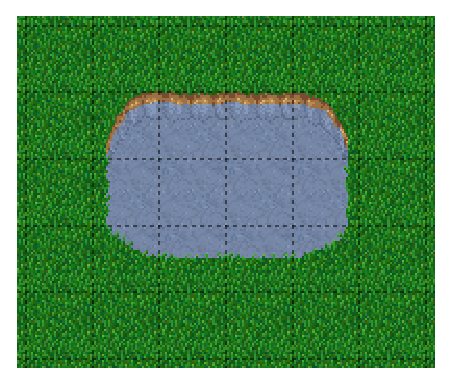
\includegraphics[scale=1]{Example/TheManaWorld/flow3.eps} &
	    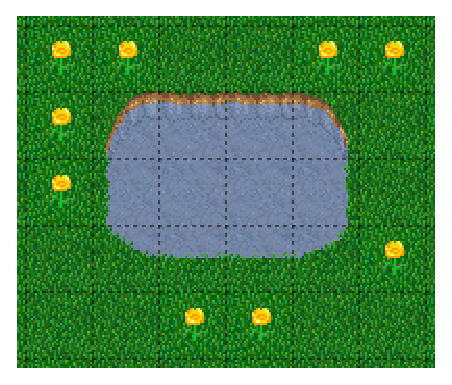
\includegraphics[scale=1]{Example/TheManaWorld/flow4.eps} \\
		\end{tabular}
  %~ \end{center}
  \caption{Series of rules get applied to build up a scenary for The Mana World. Upper left picture shows our input.
  Upper right picture shows all straigt shorelines applied. Lower left also added the bent shorelines. Lower right picture is the final version.}
\end{table}

The Mana world examples will demonstrate quite a lot of different Automapping
features. At first a shoreline will be constructed, by first adding all
the straight parts and afterwards another rule will correct the corners
to make them also fit the given tileset. After the shoreline has been added,
the waters will be marked as unwalkable for the game engine. Last but not least
some random placed fancy flowers will make the scenary even more beautiful.


\newpage
\subsection{basic shoreline} \label{basic_shoreline}
\begin{wrapfigure}{r}{0.45\textwidth}
  %~ \begin{center}
       \begin{tabular}{|c|l|}
       \hline
       tile layer & name \\
       \hline
       \hline
		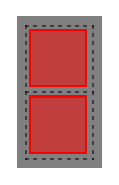
\includegraphics[scale=1]{Example/TheManaWorld/shorelinestraight/regions.eps} & regions \\
		\hline
		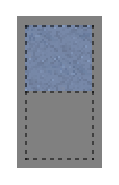
\includegraphics[scale=1]{Example/TheManaWorld/shorelinestraight/input.eps} & input\_Ground\\
		\hline
		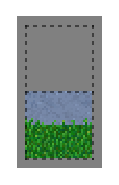
\includegraphics[scale=1]{Example/TheManaWorld/shorelinestraight/output.eps} & output\_Ground\\
		\hline
		\end{tabular}
  %~ \end{center}
  \caption{The region tile layer(top), the input tile layer(mid) and the output tile layer(bottom)}
  \label{shorelinestraight}
\end{wrapfigure}
This example will demonstrate how a straight shoreline can easily be setup 
between shallow water grass tiles. In this example we will only implement the
shoreline, which has grass in southern and water in northern direction.

So basically the meaning we will define in the input region is 
\emph{All tiles which are south of a water tile and are no water tiles itself,
will be replaced by a shoreline tile}

The region in which this Automapping rule should be defined is of 2 tiles in height and 
1 tile in width. Therefore we need a layer called \emph{regions} and it will have 2 tiles placed
to indicate this region. In figure~\ref{shorelinestraight} the top graphics shows such a region
layer.

The input layer called \emph{input\_Ground} is depicted in the middle of 
figure~\ref{shorelinestraight}. Only the upper tile is filled by the water
tile. The lower tile contains no tile. It is not an invisible tile, just no
tile at all. 

And whenever there is no tile in a place within the rule regions in an input layer,
what kind of tiles will be allowed there? There will be allowed any tiles except 
all used tiles within all input layer with the same index and name.

Here we only have one tile layer as an input layer carrying only the water tile.
Hence at the position, where no tile is located, all tiles except that water tile
are allowed.

The layer in top of 

\newpage
\subsection{Corners on a shore line}\label{example_tmw_grass_water_corners}
\begin{wrapfigure}{r}{0.6\textwidth}
  \begin{center}
		\begin{tabular}{c c c}
		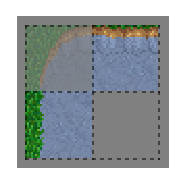
\includegraphics[scale=1]{Example/TheManaWorld/shorelinecorners/pattern0.eps} & 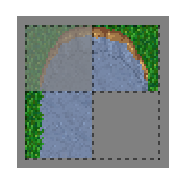
\includegraphics[scale=1]{Example/TheManaWorld/shorelinecorners/pattern1.eps} & 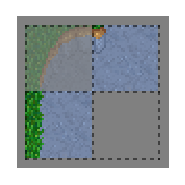
\includegraphics[scale=1]{Example/TheManaWorld/shorelinecorners/pattern2.eps} \\
		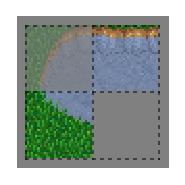
\includegraphics[scale=1]{Example/TheManaWorld/shorelinecorners/pattern3.eps} & 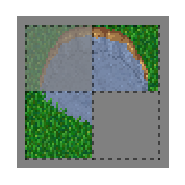
\includegraphics[scale=1]{Example/TheManaWorld/shorelinecorners/pattern4.eps} & 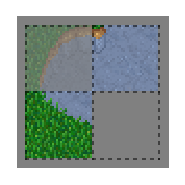
\includegraphics[scale=1]{Example/TheManaWorld/shorelinecorners/pattern5.eps} \\
		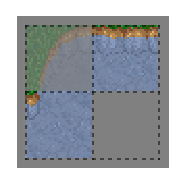
\includegraphics[scale=1]{Example/TheManaWorld/shorelinecorners/pattern6.eps} & 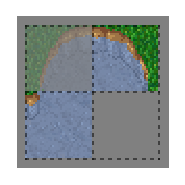
\includegraphics[scale=1]{Example/TheManaWorld/shorelinecorners/pattern7.eps} & 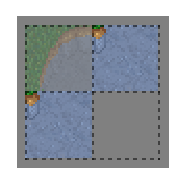
\includegraphics[scale=1]{Example/TheManaWorld/shorelinecorners/pattern8.eps} \\
		\end{tabular}
  \end{center}
  \caption{All possible inputs patterns due to other corners in the shoreline.}
  \label{shoreline_corners_needed_inputs}
\end{wrapfigure}

This example is a continuation of example~\ref{basic_shoreline}.
Now the corners of the given shoreline should be implemented automatically.
Within this paper we will just examine the bent in corner shoreline in the topleft corner.
The other shoreline corners, either bent in or bent out are constructed the same way
\footnote{Apart from some rotation and using other tiles of course.}.

So after the example~\ref{basic_shoreline} has finished, we would like to have the
corners of the shoreline get suitable tiles. Since we rely on the other example
being finished, we will put the rules needed for the corners into another new
rulefile. (which is listed afterwards in the rules.txt)

The shoreline may have some more corners nearby, which means there may be
more different tiles than the straigt corner lines. In figure~\ref{shoreline_corners_needed_inputs}
we see all inputs which should be covered.
The interesting parts are all in the red squares. Outside the red squares
it is just continued to have a niver look.

Both the tiles in the top right corner and in the lower left corner are
directly adjacent to the desired (slightly transparent) tile in the top left
corner.

We can see 3 different tiles for the lower left corner, which is
straight shore line, bent inside and bend outside shore lines.

Also we see 3 different inputs for the top right corner, which also
is straight, bent in or out shore line.

\subsubsection{regions}

\begin{wrapfigure}{r}{0.60\textwidth}
  \begin{center}
       \begin{tabular}{c c c}
		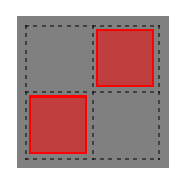
\includegraphics[scale=1]{Example/TheManaWorld/shorelinecorners/regions_input.eps} & 
		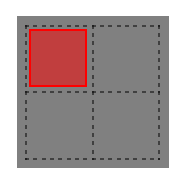
\includegraphics[scale=1]{Example/TheManaWorld/shorelinecorners/regions_output.eps} & 
		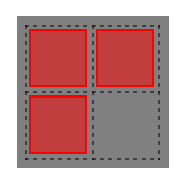
\includegraphics[scale=1]{Example/TheManaWorld/shorelinecorners/regions_united.eps} \\
		\end{tabular}
  \end{center}
  \caption{Input regions (left) and output regions (mid) and the combination of both(right)}
  \label{shoreline_corners_regions}
\end{wrapfigure}
So with this rule we want to put the bent in shore line tile in the top
left corner, hence we don't care which tile has been there before.
Also we don't care about the tile in the lower right corner. (probably water,
but can be any decorative watertile, so just ignore it).

Therefore we will need different input and output regions. In the figure~\ref{shoreline_corners_regions}
we can see the both tilelayers $\textup{regions}\_\textup{input}$ and
$\textup{regions}\_\textup{output}$. The input section covers just these
two tiles as we discussed. The output region covers just the single tile
we want to output. Though the input and output region do not overlap,
the united region of both the input and the output region is still one coherent
region, so it's one rule and works\footnote{output regions can be larger
than absolutely required, since when there are no tiles in the output section,
the tiles in the working map are not overwritten but just kept as is, hence
the output region could also be sized as the united region of both the
output and input region.}.

\newpage
\subsubsection{input layers}
\begin{wrapfigure}{r}{0.45\textwidth}
		\begin{tabular}{|c|l|}
		\hline
		tile layer & layer name  \\
		\hline
		\hline
		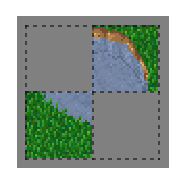
\includegraphics[scale=1]{Example/TheManaWorld/shorelinecorners/input_Ground2.eps} & input\_Ground \\
		\hline
		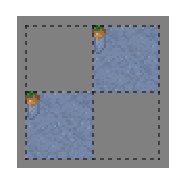
\includegraphics[scale=1]{Example/TheManaWorld/shorelinecorners/input_Ground1.eps} & input\_Ground \\
		\hline
		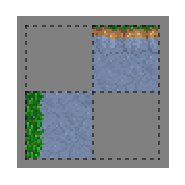
\includegraphics[scale=1]{Example/TheManaWorld/shorelinecorners/input_Ground.eps} & input\_Ground \\
		\hline	
		\end{tabular}
		\caption{All the input layer for the rule defining one corner for the shoreline.}
		\label{shorelinecorner_inputsection}		
\end{wrapfigure}
Now we want to put all the nine possible patterns we observed as possible
input for this rule. We could of course define nine different layers
$\textup{input}1  \_\textup{Ground}$ up to
$\textup{input}9  \_\textup{Ground}$
Nine TileLayers?! what a mess, we'll put it in a better way\footnote{
Also consider not having just 3 possible tiles at the 2 locations but 4.
Then we would need 4*4=16 tilelayers to get all conditions. Another downside
of this comes with more needed locations:
Think of more than 2 locations needed to construct a ruleinput. So for 3
locations, then each location could have the 3 possibilites, hence you need
3*3*3 = 27 tilelayers. It's not getting better...}


Since the rules are constructed on a per-tile basis, we only need 3 tilelayers
for the input section all of them having the same $\langle \textup{index} \rangle$,
hence the same name $\textup{input}\_\textup{Ground}$.
We need to make sure that in both positions all of each the three possible
tiles are placed. In figure~\ref{shorelinecorner_inputsection} we see the three input layers,
which match all the 9 possibilites as mentioned in figure~\ref{shoreline_corners_needed_inputs}.

\subsubsection{output}



The output is straight forward, since only one tile is needed. 
No randomness is needed, hence the $\langle \textup{index} \rangle$ is not needed to be varied, so it's kept empty.
The desired output layer is called $\textup{Ground}$, so the overall name of the single output layer
will be $\textup{output}\_\textup{Ground}$. At this single layer at the correct location the correct tile 
is placed\footnote{See top left corner in the red boxes of figure~\ref{shoreline_corners_needed_inputs}}.

\subsubsection{summary}
The table~\ref{shorelinecorner_complete} shows all layers needed for the rule, which adds corners to the shoreline in The Mana World
\begin{table}
		\begin{tabular}{|c|l|c|l|}
		\hline
		tilelayer & layer name & tilelayer & layer name\\
		\hline
		\hline
		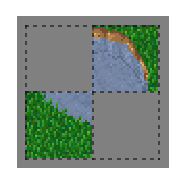
\includegraphics[scale=1]{Example/TheManaWorld/shorelinecorners/input_Ground2.eps} & input\_Ground & 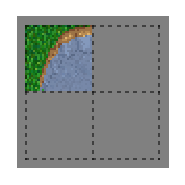
\includegraphics[scale=1]{Example/TheManaWorld/shorelinecorners/output_Ground.eps} & output\_Ground \\
		\hline
		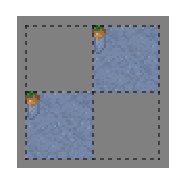
\includegraphics[scale=1]{Example/TheManaWorld/shorelinecorners/input_Ground1.eps} & input\_Ground & 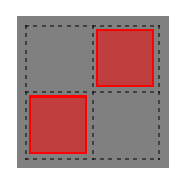
\includegraphics[scale=1]{Example/TheManaWorld/shorelinecorners/regions_input.eps} & regions\_input \\
		\hline
		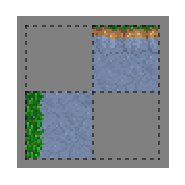
\includegraphics[scale=1]{Example/TheManaWorld/shorelinecorners/input_Ground.eps} & input\_Ground & 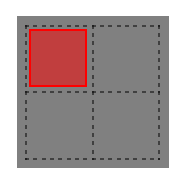
\includegraphics[scale=1]{Example/TheManaWorld/shorelinecorners/regions_output.eps} & regions\_output\\
		\hline		
		\end{tabular}
		\caption{The complete Automapping rules file defining one corner for the shoreline.}
		\label{shorelinecorner_complete}
\end{table}

